\documentclass[11pt, oneside]{article} 
\usepackage{geometry}
\geometry{letterpaper} 
\usepackage{graphicx}
	
\usepackage{amssymb}
\usepackage{amsmath}
\usepackage{parskip}
\usepackage{color}
\usepackage{hyperref}

\graphicspath{{/Users/telliott_admin/Tex/png/}}
% \begin{center} 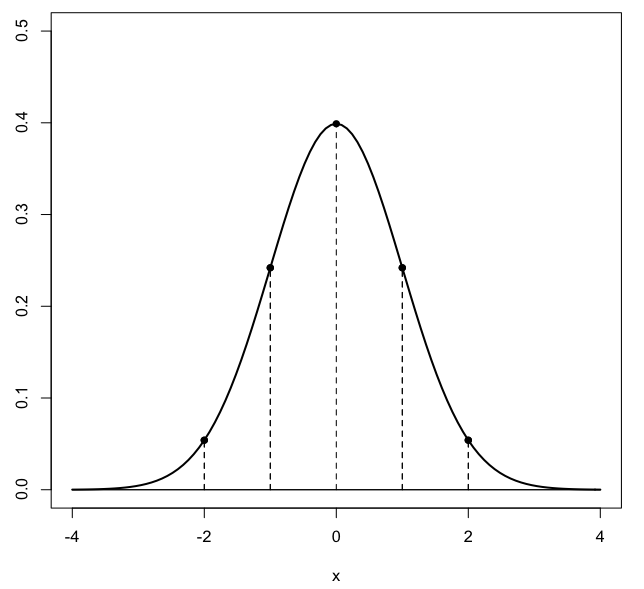
\includegraphics [scale=0.4] {gauss3.png} \end{center}

\title{Orthocenter}
\date{}

\begin{document}
\maketitle
\Large
An altitude of a triangle is a line extended from a vertex so as to form a right angle with the opposing side.  The orthocenter is the point where the three altitudes of a triangle meet.

Assume for now that the three altitudes \emph{do} meet at a single point, we will come back to this question later.
\begin{center} 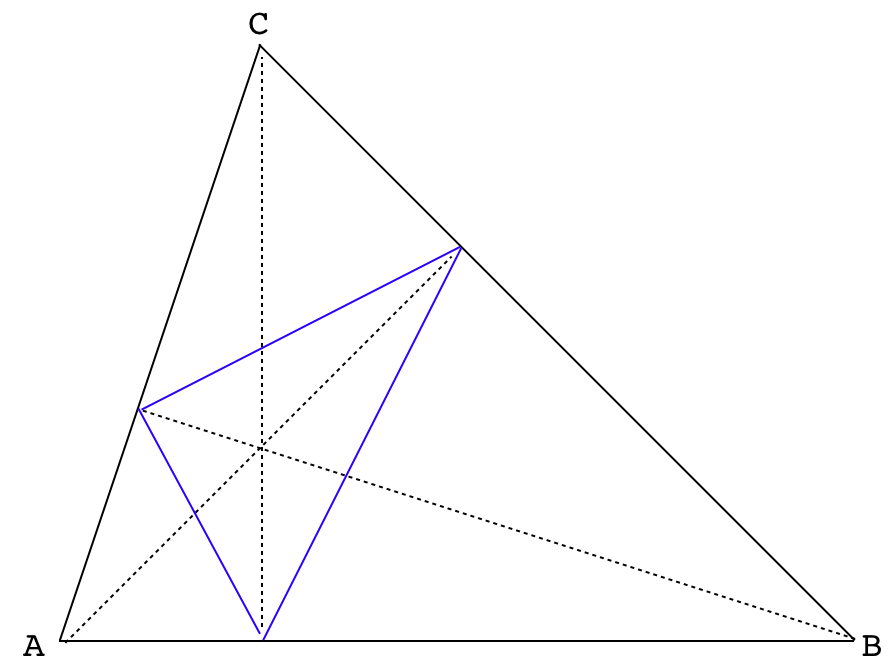
\includegraphics [scale=0.25] {ortho1.png} \end{center}
The altitudes are drawn as dotted lines in the figure above.  The points where these lines meet their opposite sides have also been connected, forming another triangle outlined in blue.

The same construction for the centroid, formed from lines that bisect the opposing sides, gives four small triangles which are all congruent.  In the case of the orthocenter, we will show that the three outer triangles are similar (though obviously not congruent), while the one in the center is different.

The first observation is that the angles $A$, $B$, and $C$ are divided by the altitudes into two parts with the measures repeated as shown below.  

\begin{center} 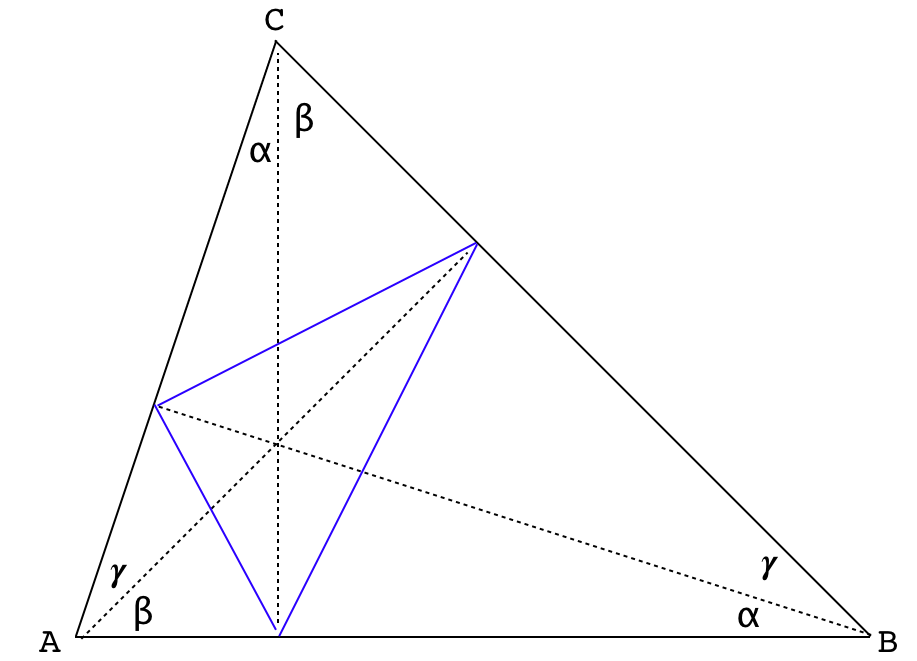
\includegraphics [scale=0.25] {ortho2.png} \end{center}

Proof:  there are two right triangles formed that include $A$ as a base angle.  The corresponding complementary angles must be equal, and these are labeled $\alpha$.  A similar argument gives $\beta$ and $\gamma$.

Switching our attention to the central angles, we can show that these have measures equal to the vertices.
\begin{center} 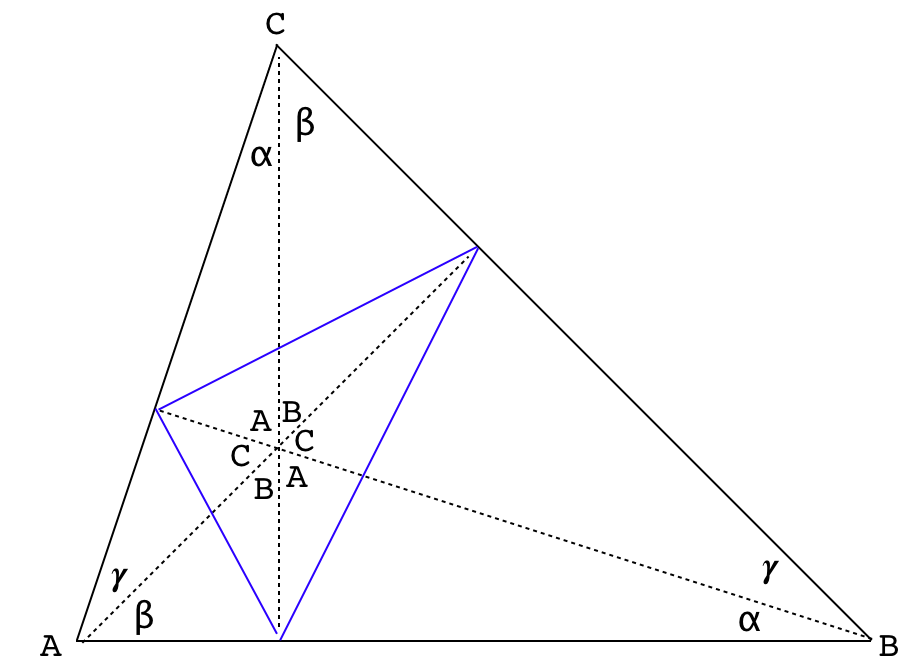
\includegraphics [scale=0.25] {ortho3.png} \end{center}

The argument builds on the one above, each central angle is part of a right triangle with one of $\alpha$, $\beta$, or $\gamma$ as the complementary angle.

\subsection*{angle bisectors}
The next fact we need is that the altitudes are angle bisectors for the inscribed triangle.   

Here is a neat and quick proof from Courant and Robbins.  
\begin{center} 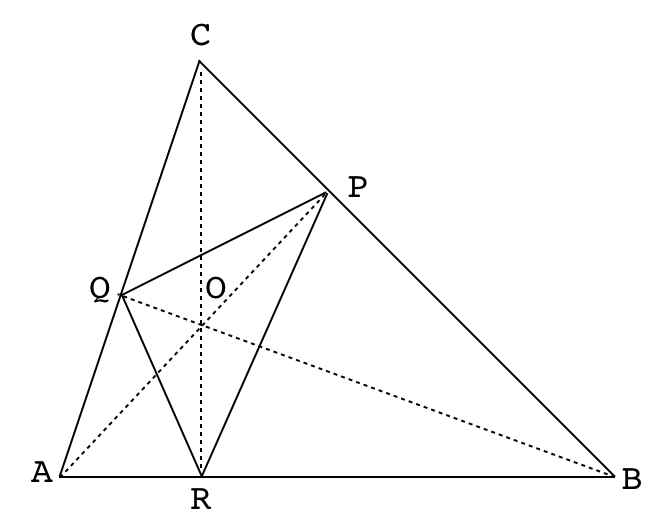
\includegraphics [scale=0.3] {ortho11.png} \end{center}
Label the vertices of the altitudes as $P,Q,R$ and the orthocenter as $O$.  Since $\angle OPB$ is a right angle and so is $\angle ORB$, the quadrilateral $OPBR$ containing both can be inscribed into a circle with $OB$ as the diameter.

\begin{center} 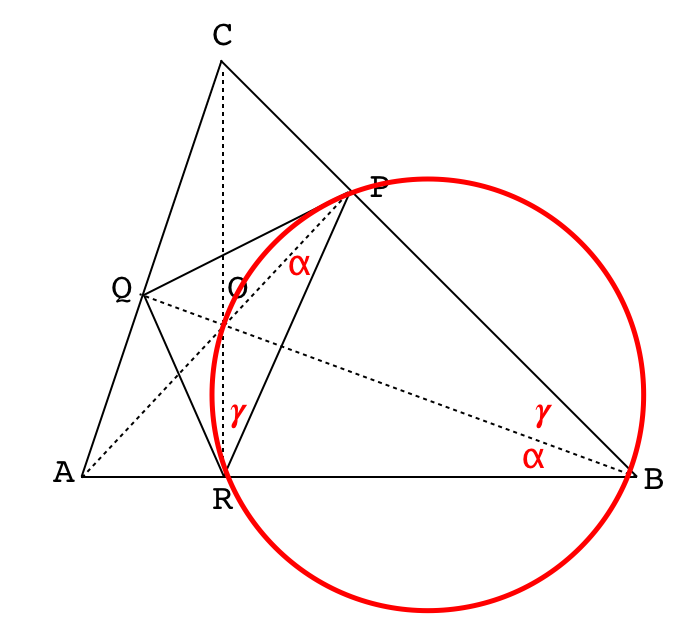
\includegraphics [scale=0.3] {ortho12.png} \end{center}
Now, we use the theorem that if two angles on the circumference of a circle sweep out the same arc, they are equal to each other  This allows labeling of $\alpha$ and $\gamma$ as shown.  

Then, since $A$ is the complement of $\alpha$, and $C$ is the complement of $\gamma$, we obtain

\begin{center} 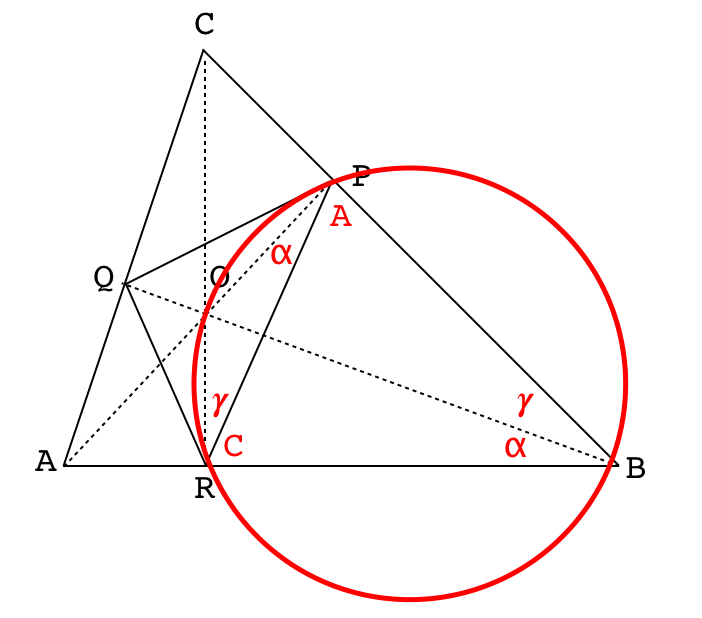
\includegraphics [scale=0.3] {ortho14.png} \end{center}

We could draw two more circles, but instead just invoke symmetry:

\begin{center} 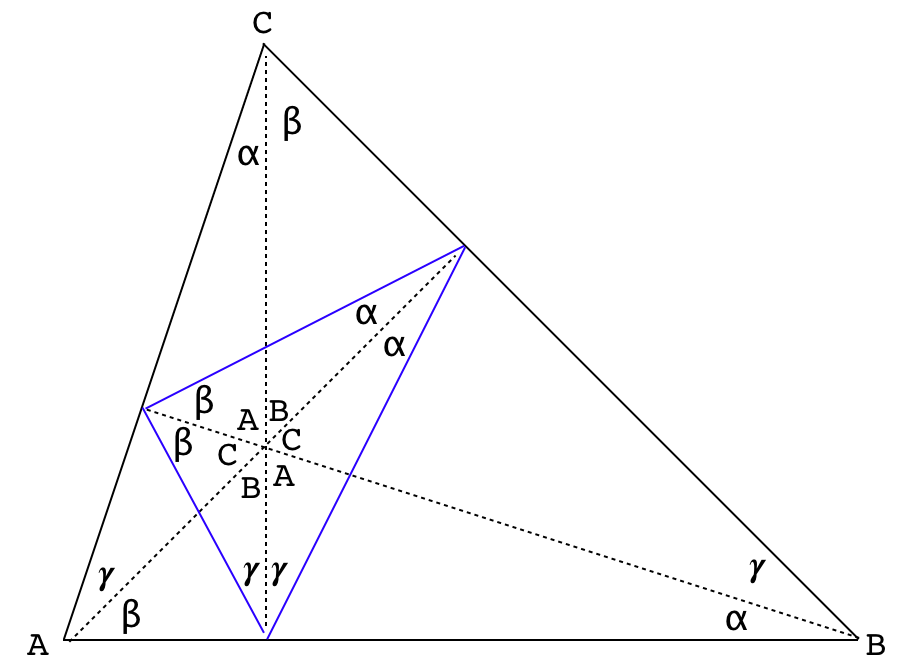
\includegraphics [scale=0.3] {ortho15.png} \end{center}

So finally, we have
\begin{center} 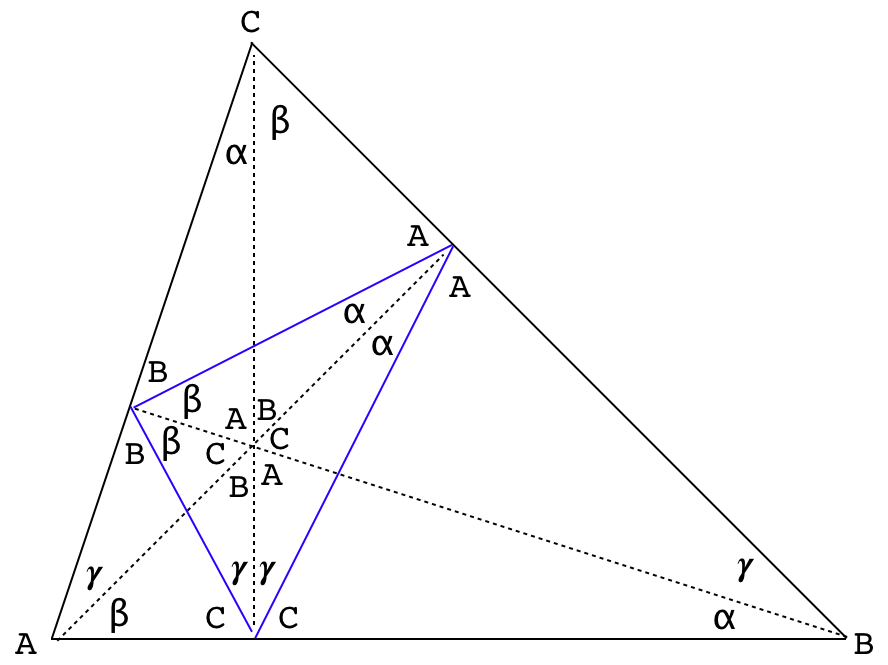
\includegraphics [scale=0.3] {ortho16.png} \end{center}

Thus, we have established that the altitudes are angle bisectors for the included triangle, and that the three small outer triangles are congruent, by AAA.

\subsection*{Orthocenter exists}
For the above derivation, we assumed that the three altitudes do indeed meet at a single point.  This is a direct consequence of Ceva's Theorem, which we've seen before.  

Below we give an alternative proof, due to Euler, which is stunning, following

\url{https://artofproblemsolving.com/wiki/index.php/Orthocenter}

Borrowing their figure:
\begin{center} 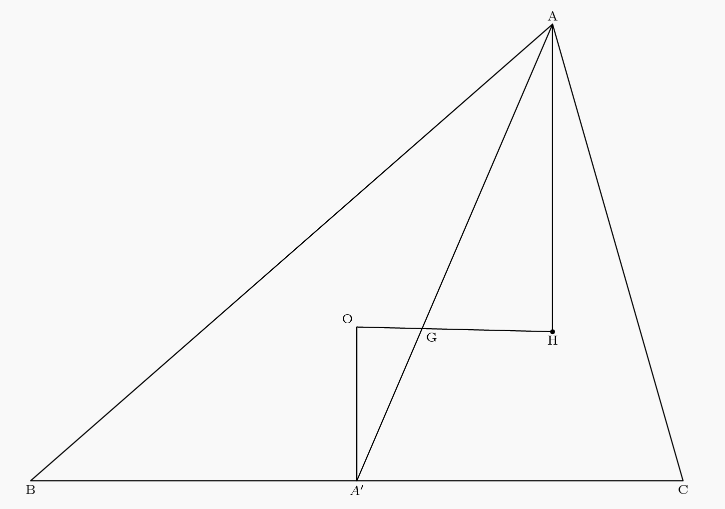
\includegraphics [scale=0.4] {circumcenter.png} \end{center}
The orientation is reversed from what we had above.  First, the point $O$ is the circumcenter of the triangle:  the center of the circle which contains all three vertices of the triangle.  

Clearly, this circle  has a center.  The classic construction is to bisect each side (here $BC$ is bisected at $A'$), and erect a perpendicular.  The point where the three perpendiculars cross is the circumcenter, which is the center of the circle.  

\begin{center} 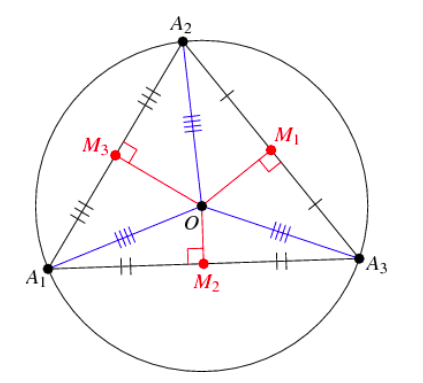
\includegraphics [scale=0.45] {three_point_circle2.png} \end{center}

So, assume we have done this and that point is $O$.

The next point, $G$, is the centroid.  One way to find this point is to draw all three lines connecting vertices with the midpoints of the opposite side ($AA'$).  However, if you recall, the distance from the vertex $A$ to $G$ is twice the distance from the midpoint $A'$ to $G$.  Hence we draw point $G$ using arithmetic.

Now, extend $OG$ by twice its length, to $H$.  ($2OG = GH$).
\begin{center} 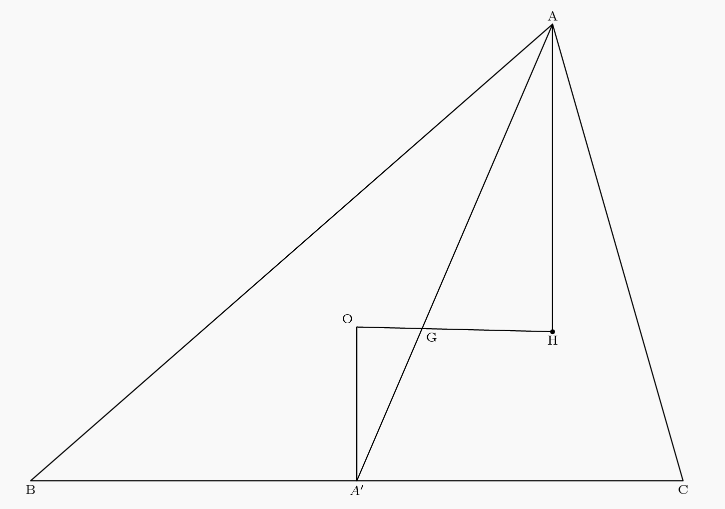
\includegraphics [scale=0.4] {circumcenter.png} \end{center}
Because $AG$ is twice $A'G$ and $GH$ is twice $OG$ and the two triangles share both angle $\angle OGA'$ (equal to $\angle AGH$), they are similar triangles.  

Since $\angle A'OG$ is a right angle, therefore so is $\angle AHG$.  This means that $AH$ is perpendicular to $BC$.  Thus, $AH$ is a part of the altitude from $A$ to $BC$ (the whole altitude is not shown).

The same construction could be done for the other two vertices, each time ending at $H$.  This shows that $H$ is unique, and that $H$ is on all three altitudes.

This proof also demonstrates that the orthocenter, centroid and circumcenter lie on a single line, and that the distance from centroid to orthocenter is twice that from centroid to circumcenter.
 
\end{document}